\documentclass[a4paper, 12pt, pagesize, parskip=half-]{scrartcl}

\usepackage{fontspec}
\defaultfontfeatures{Ligatures=TeX}
\usepackage{polyglossia}
\setmainlanguage{german}
\usepackage{fixltx2e}
\usepackage{microtype}
\usepackage{selnolig}
\usepackage{graphicx}
\usepackage[unicode]{hyperref}

\pagestyle{empty}

\begin{document}
\begin{center}
	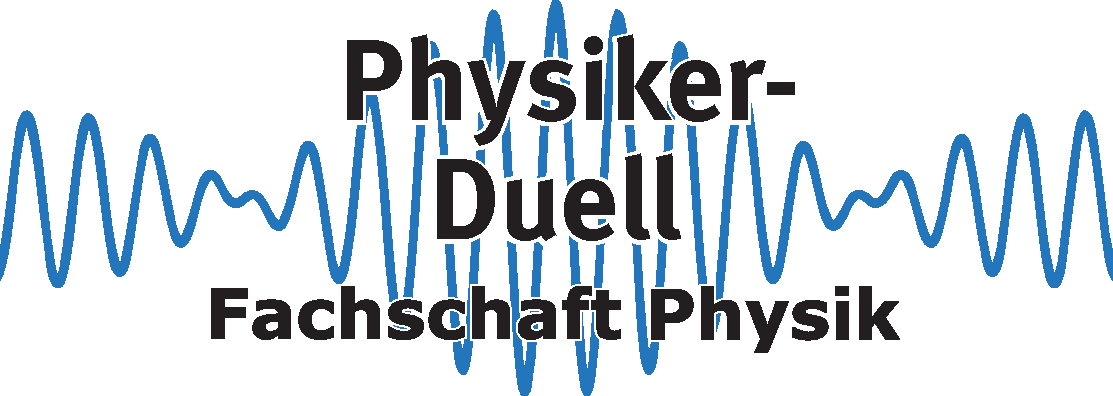
\includegraphics[width=\textwidth]{Physikerduell_Logo.pdf}
\end{center}

\bigskip

Am Donnerstag, den 18.06., findet das Sommerfest am Fachbereich Physik (organisiert von der Fachschaft
Physik) statt. Im Rahmen des am selben Tag um 16:15 Uhr stattfindenden Allgemeinen Physikalischen
Kolloquiums wird als Teil des Sommerfests auch wieder das Physiker-Duell stattfinden.

Basierend auf den Regeln der bekannten Fernsehsendung „Familien-Duell“ messen sich in diesem
rasanten Quiz verschiedene Arbeitsgruppen des Fachbereichs Physik im direkten Wettstreit.
Nur eine von ihnen kann am Ende triumphieren und den Pokal als Beweis für ihre Überlegenheit
gegenüber ihren Kollegen mit in die eigenen Büros tragen.

Zu verschiedenen (mehr oder weniger absurden) Fragen wurden „100 Physiker befragt“. Die Aufgabe
der Arbeitsgruppen im Duell ist es, jene Antworten zu erraten, die auch die meisten der Befragten
gegeben haben. Doch das kann auch nach hinten losgehen: Nach drei falschen Antworten hat das
gegnerische Team die Möglichkeit, mit nur einer richtigen Antwort alle bereits erspielten
Punkte der Runde zu stehlen! In späteren Runden sind die Antworten zudem ein Vielfaches wert.
Die Duelle bleiben also bis zum Ende spannend – auch für weit abgeschlagene Teams kann sich
das Blatt noch im letzten Moment wenden!

Hier noch einmal die wichtigsten Daten:

\bigskip
\Large
\begin{tabular}{lp{12.5cm}}
\textbf{Was?}	& Physiker-Duell \\
\textbf{Wann?}	& 18.06.2015, 16:15 Uhr \\
\textbf{Wo?}	& HS 2 (IG 1) \\
\textbf{Wer?}	& Arbeitsgruppen des Fachbereichs und die Fachschaft (und jeder, der zusehen möchte) \\
\end{tabular}
\end{document}